% !TEX TS-program = latex
\documentclass[a4paper,12pt]{report}
\newcommand{\ra}[1]{\renewcommand{\arraystretch}{#1}}
\usepackage{amsmath}
\usepackage[mathscr]{eucal}
\usepackage{amssymb}
\usepackage{indentfirst}
\usepackage{latexsym}
\usepackage{hyperref}
\usepackage{setspace}
\usepackage{enumerate}
\usepackage{pdfpages}
\usepackage{url}
\usepackage{verbatim}
\usepackage{booktabs}
\usepackage{color}
\usepackage{epsfig}
\usepackage{longtable}
\usepackage{tabularx}
\usepackage{dcolumn}

\usepackage{float}
\usepackage{xspace}

\newcommand{\todo}[1]
{
    {\color{red}$\blacksquare$~\textsf{[TODO: #1]}~$\blacksquare$}
}

\newcommand{\EditOne}[1]
{
    {\color{blue}{#1}}
}

\newcommand{\K}{{\tt Kepler}}


\bibliographystyle{plain}
\textwidth=14.945cm
\oddsidemargin=0.5cm
\evensidemargin=0.5cm

\begin{document}
\doublespacing

\begin{titlepage}
\vspace*{2cm}
\noindent
\begin{flushleft}
	\setlength{\baselineskip}{2\baselineskip}
	{{\Huge \bf Automatic Classification of Kepler Planetary Transit Candidates Using Multilayred Neural Networks}}
\end{flushleft}


\vspace{1cm}
\vspace{\fill}
\vspace{1.3cm}
\begin{tabbing}
mmmmmmmmmmmmmmmmm\= \kill
\>Prabath Peiris\\
\>Capstone Project Proposal\\
\>Machine Learning Nanodegree\\
\>Udacity\\
\> \\
\end{tabbing}
\end{titlepage}

\thispagestyle{empty}
\newlength{\origpar}
\setlength{\origpar}{\parindent}
\setlength{\parindent}{0pt}
%\input{Abstract/abstract}
\setlength{\parindent}{\origpar}
\thispagestyle{empty}
\tableofcontents
\clearpage

\renewcommand {\baselinestretch} {1.0}
\pagebreak
%\pagenumbering{arabic}


\chapter{Domain Background}

Kepler is a space observatory launched by NASA in 2009 to discover Eath-sized exoplanets orbiting other stars  \cite{2010ApJ...713L..87J}. Kepler mission developed several decades to answer the centuries-old question: How frequent are other Earth-like planets in Milkyway galaxy? In particular, what is the frequency of Earth-size planets in the Habitable-Zone of solar-like stars? There are three different types of exoplanets are common in our universe: gas giants, hot-super-Earths in short period orbits, and ice giants. The challenge is to find the terrestrial planets that are in the habitable zone of their stars where liquid water might exist on the surface on the planet.

The scientific objective of the Kepler mission is to explore the structure and diversity of planetary systems. This mission surveys a large sample of stars to determine the percentage of terrestrial and large planets that are in or near the habitable zone of a wide variety of stars and determine the distribution of size and shapes of the orbits of these planets. Kepler mission also estimates how many planets are in multiple-star systems. After collecting a large number of data points, using many techniques scientists determine the properties of those stars that harbor planarity systems including the planets itself. 

\section{Scentific Goals and Objectives of the Kepler Mission}

The primary goal of the Kepler Mission is to survey our region of the Milky Way galaxy to discover hundreds of Earth-size or larger planets in or near the habitable zone of solar-like stars and determine the existence of solar system like planetary systems \cite{2014PNAS..11112647B}. The scientific objective of the Kepler Mission is to explore the structure and diversity of extrasolar planetary systems. This is achieved by observing a large sample of stars to:
\begin{itemize}
  \item Determine the frequency of terrestrial and larger planets in or near the habitable zone of a wide variety of stellar spectral types of stars. 
  \item Determine the distribution of the size of planets and the size of the planet’s orbits.
  \item Estimate the frequency of planets in multiple star systems.
  \item Determine the distributions of orbital sizes, their light reflection properties (albedo), size, and density of
short-period giant planets.
  \item Identify additional members of each photometrically discovered planetary system using complementary techniques. 
  \item Determine the properties of those stars that harbor planetary systems. The spectral type, luminosity, and composition for each star showing transits are obtained from ground-based observations.
  \item Asteroseismology analysis of the data will be used to determine the mass, age, and size of the stars and astrometric analysis of the data will be used to calculate their distances, which also is used to calculate the size of the stars.
\end{itemize}

\section{Habitable Zone}

Habitable Zone is the range in the distance from a star where liquid water could exist on the surface of a planet orbiting a star that possibly supports life. Liquid water is essential to all life on Earth, and so the definition of a habitable zone is based on the hypothesis that extraterrestrial life would share this requirement \cite{2014ApJ...787L..29K}. This is a very traditional definition, as a planet surface temperature may depend on other factors such as greenhouse gas abundance, its reflectivity, atmospheric and oceanic circulation, radioactive decay, and tidal heating within the planet. These energy sources can be easily allowed the planet to have subsurface liquid water reservoirs.  Jupiter's moon Europa has liquid water ocean tens of kilometers below its surface that may well be habitable for some organisms. More than 20 planets, including the nearest extrasolar planet, Proxima Centauri b \cite{2016Natur.536..437A}, have been found that are both roughly Earth-sized and orbiting within a habitable zoned of their stars. 

\section{The Transit Method of Detecting Extrasolar Planets}

The Kepler mission detecs exoplanets using transit photometry \cite{2000ApJ...529L..45C}. When a planet passes in front of a star as a view from Earth, the event is call a ``{\emph {transit}}''. For example, we can observe an occasional Venus or Mercury transit from Earth as a small black dot creeping across the Sun. During this transit, the transiting planet block the starlight and dips the brightness of the star. When this happen, we say the planet transit the star, and can be detect using transit phometry. During transit, raw data is collected in the form of a sequence of stellar images, which are processed in to "light-curves" tracking the brightness of a star over time. Light-curves are graphs that show the brightness of an object over a period. 

\begin{figure}[!h]
\begin{center}
        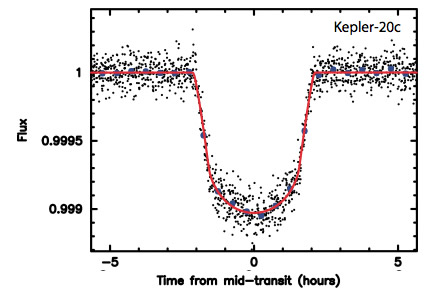
\includegraphics[width=0.6\textheight]{img/k20c.jpg}
        \caption{The light curve shown here was made from brightness data gathered by the Kepler Mission for discovery of planet Kepler-20c.
Image Credit: NASA}  \label{fig:lightcurve}
\end{center}
\end{figure}

Figure \ref{fig:lightcurve} shows the light curve made from the brightness data from Kepler Mission for the discovery of a planet named \emph{Kepler-20c}. Data clearly show the flux of the host star drop notability when the planet is in transit. This is the primary signature we are looking in the transit photometry to discover planets that are in orbits around stars. These planets create this photometric signature periodically while they are orbiting around the star. To make things more complicated, the light curves of some other objects also create similar photometric signatures: eclipsing binaries stars, certain other variable stars. During the classification stage, we need to classify these object as false positives. 


\section{Project  Proporsal and Motivation}
NASA's Kepler mission search for extrasolar planets has collected data from hundreds of thousands of star systems. Processing these large amounts of data, so far mission discovered 4,696 candidate exoplanets and 2,331 of them are confirmed as exoplanets leaving many more planet candidates to be confirmed in the dataset. These potential planetary candidates are searching using an algorithm that looks for periodic planetary transit in the light curves, but spurious intensity dips and other noise in the data due to non-planetery stellar variability has led to high false positive rates for detecting transits. As the initial planetary candidates found by this search method require extensive and costly subsequent validation, there is a need to reduce the error rate in exoplanet candidate identification. This exoplanet candidate data set refer to as Kepler Object of Interest (KOI). I present an algorithm (Multilayered Neural Network - MNN) to classify KOI as confirmed exoplanets or false positives using publically available data. MNN uses previously generated features extracted from the lightcurve time-series data, as well as newly generated autocorrelation features derived from the time-series specifically during the planet transits. 

NASA launched the Kepler mission when I was an undergraduate student (Physics major) in 2009. Since the day the mission has been initiated, I closely follow the mission updates.  I have moved to upstate NY to pursue my graduate studies in theoretical astrophysics (MS thesis in Numerical Relativity). Durig this time I have attended numerous scientific talks given by Kepler fellowship researchers at the University explaining and exploring the Kepler dataset. There are some groups are already using machine learning techniques to classify the Kepler data while others are developing more manual and careful procceses to extract planetary candidates. After taking the Udacity machine learning nano degree, it is natural for me to think of applying machine learning techniques to the Kepler dataset and see if that can improve the classification of planetary candidates. 

\chapter{Problem Statement}

Kepler is a single instrument spacecraft that collect most contiguous and long-running photometric time series possible. Kepler has the capability to observe approximately 170,000 stars simultaneously while it is operating. The fundamental objective of the Kepler mission is to detect a large number of transiting exoplanets. The ultimate goal of the primary mission was a characterize the frequency of exoplanets on diameter, orbital period and host star.  The Manual classification of the findings of Kepler object has proven very time-consuming. The new space-based, transit photometry missions such as K2 \cite{2014PASP..126..398H}, TESS \cite{2014SPIE.9143E..20R}, and PLATO 2.0 \cite{2014ExA....38..249R} also produce a large number of the dataset that demands some level of automation to do the classification. 

Using machine learning classification techniques, we can speed up the process and provide a more continuous rating of planarity candidates. There are various of machine learning classification techniques has been applied to Kepler dataset including random forests, SVM, K-mean clustering \cite{2015ApJ...800...99T, 2015ApJ...806....6M}.  In this project, we are attempting to train a Multilayered Neural Network to identify the potential planetary candidates in the Kepler dataset. 

\chapter{Datasets and Inputs}

\section{Kepler Pipeline}

The Kepler Pipeline \cite{2010ApJ...713L..87J} is a data reduction pipeline used for translating the Kepler raw pixel data into possible transiting planet detections. Kepler mission perform photometric observations of carefully selected stars (around 156,000) using its 115 deg$^2$ field of view (FOV) as reviewed in Borucki et el. (2010) \cite{Borucki977}
 and Koch et al. (2010)  \cite{2010ApJ...713L..79K}. The Kepler Mission Science Operations Center (SOC) at NASA Ames Research Center performs major functions on these datasets including calibrate CCD array, download data (light curves) from the spacecraft periodically, remove systematic noise \cite{2012PASP..124.1000S} and perform statistical tests to reject false positives and establish accurate statistical confidence in each detection.

\begin{figure}[!h]
\begin{center}
        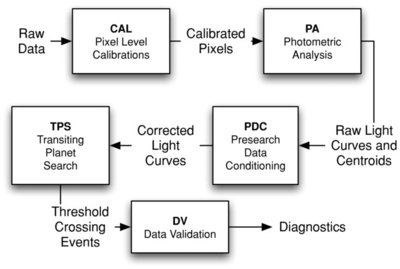
\includegraphics[width=0.5\textheight]{img/kpipeline.jpg}
        \caption{Data flow diagram for the SOC Science Pipeline. Image Credit: The American Astronomical Society}  \label{fig:kpipleline}
\end{center}
\end{figure}

Figure \ref{fig:kpipleline} show the major steps and modules of the pipeline. In particular the last two modules of the pipeline; those that identify as Threshold Crossing Events (TCEs) and their subsequent transit model fiting. TCE is a sequence of significant, periodic, planet transit-like features in the light curve of a target star. Transiting Planet Search module take takes as input the systematic error-correlated light curve for a star and searches a parameter space of possible transit signatures and outputs a TCE or say that does not exists TCE event on the target star. This produce smaller subset of target stars what is given to the Data Validation (DV) module. DV module takes initial TCE and gaps the transit signatures from the light curve and uses the Transiting Planet Search to find additional TCEs on the same target star. This process repeats until it finds all the TCEs on given star. More details on this process explained by Mandel and Agol (2002) \cite{2002ApJ...580L.171M} and Claret and Bloemen (2011) \cite{2011yCat..35290075C}.

TPS algorithm detects transit-like features in light curves by applying noise compensating, wavelet-based matched filtering. TPS characterized the power spectral density (PSD) of the observation noise as a function of time to implement a whitening filter in the wavelet domain. The trial transit pulse is whitened and correlated against the whitened flux time series. Features with correlations above the threshold of 7.1$\sigma$ are flagged as potential threshold crossing events and subjected to additional tests in TPS to guard against false alarms.

Algorithm searches a parameter space with varying transit durations $D$ and produce a Single Event Statistics (SES) time series that is the significance of the detection of the reference transmit pulse centered at that particular time for each $D$

\begin{equation}\label{eq:ses}
	SES(t) = N(t) /\sqrt{D(t)}
\end{equation}

$\sqrt{D(t)}$, is the expected signal to noise ratio of a signal that exactly matches the template pulse and $N(t)$ is the correlated time series.



Multiple Event statistics (MES) is constructed that characterizes a significant detection in a search over varying orbital period $p$ and epochs (phase) $t_0$ by folding $N(n)$ and $D(n)$. MES  $>$ 7.1$\sigma$ may produce a TCE if it also passes additional statistical tests. SES and MES are the basis of some of the attributes used in the training set.


\section{KOI and TCE Sttributes }

The Threshold Crossing Events (TCE) catalog contain a sequence of transit-like features in the flux time series of a given target star. These TCE data can download from NASA Exoplanet Archive databases \footnote{\url{http://exoplanetarchive.ipac.caltech.edu/cgi-bin/TblView/nph-tblView?app=ExoTbls&config=q1_q17_dr24_tce}}, and also the detail description of the table fields \footnote{\url{http://exoplanetarchive.ipac.caltech.edu/docs/API_tce_columns.html }} are listed as public data. Kepler Object of Interest (KOI) catalog contains object data including many attributes. The detail attributes are listed on NASA Exoplanet Archive website \footnote{\url{
http://exoplanetarchive.ipac.caltech.edu/docs/API_kepcandidate_columns.html}}, and dataset can be download from the arcive tables \footnote{\url{http://exoplanetarchive.ipac.caltech.edu/cgi-bin/TblView/nph-tblView?app=ExoTbls&config=cumulative}}. All these data cab be download as bulk using data tools available in the archive website.

\section{Some Important Attributes}
\label{label:important_attributes}
There are a large number of attributes available in the KOI and TCE datasets. Out of these attributes, following attributes has significant importance in classification process according to the literature. We will be including these attributes along side with other attributes that will be determined by using Independent Component Analysis.

\begin{itemize}
	\item $MES_{max}$/$MES_{min}$
	\item SNR (for all-transit model fit)
	\item MES scaled by SES auto-correlation statistics
	\item $\chi^{2}$ statistics for the all-transits model fit
	\item Ratio of the planet's semi-major axis to stellar radious
	\item The proportion of the light curve that was missing during this TCEs transit
\end{itemize}

\section{Missing Attributes}
In some circumstances, there are missing attributes in the dataset due to missing information in the stellar catalogs; the data validation fit fails to converge, or a processing timeout is reached. These missing attributes can be fill using reasonable methods such as mean, median, and in case of missing stellar attributes can be filled using sun's parameters. These various substitutions will be tested when training the network.

\section{Classification Labels}

Each Threshold Crossing Event (TCE) is subject to a vetting process performed by the Kepler TCE Review Team (TCERT). During the triage (Initial) vetting stage, all TCEs are partition into two different sets: Problematic Ligh Curves that has instrumental noise and Kepler Object of Interest. KOI is a TCE that contains convincing transit-like features that do not present obvious evidence that the TCE was generated from non-transiting phenomena such as instrumental noise. These KOIs moves to next level of the vetting process performed by individuals manually inspecting light curves using detection statistics. Any indication they see the signal came from an eclipsing binary star or more complex forms of instrumental noise removed from the list. TCEs that survive this removal process are classified as Planet Candidates (PC).


We can identify three different types of classification labels in the processed dataset: Planetary Candidates (PC), Astrophysical False Positives (AFP) and non-transiting phenomena (NTP). PCs are confirmed as planets, statistically validated as planets or determined to be a planet candidate by the TCERT. AFPs are those TCEs that have been shown to be eclipsing binary stars or have shown evidence that the transiting object being detected is not located around the target tart. NTP are those TCEs that failed the initial vetting process.

I am planning to use machine learning algorithm (Neural Network) to find a function that maps attributes produced by the Kepler Pipeline for each TCE to a classification label of PC, AFP or NTP. This classification funtion is purely based on the statistical distributions of the attributes for each TCE and the algorithm does not attempt to physically model the process of the planet transit beyond what is already present in the TCE attribute catalogs.

\chapter{Solution Statement}


Machine learning techniques contribute a way to automate some step of exoplanet discovery. The TCE vetting process is a tedious and time-consuming (mostly a manual) process. Modern astronomical observational instruments generate a large amount of data within a short period of observational time. These observations may contain such a crucial events that need future follow-up observations using other telescopes (using other wavelengths); hence, processing these time series data and extracting meaningful information is a time sensitive process. Solution to this is to process Kepler data using machine learning algorithms to express the classification while reducing human errors. I am planning to use trained Neural Network to process the TCE data to make the classification. 
\chapter{Benchmark Model}

I am planning to experiment with benchmarking the neural network by performing many training trials by varying number of training data sets. For each trail $i$, the training time to obtain a correct network $t_i$ will be recorded. Trials which are not successful within a time limit $T$ will consider as failures. Initial weight will be randomly chosen \cite{hamey1991benchmarking}. 




\chapter{Evaluation Metrics}

Using Neural network classifier to make classification on Kepler TCEs is a discrete prediction machine learning problem. That is to say; the NN decide what category the given TCE belong to. There are many metrics available for us to check how well our NN is performing and I am planning to use couple of these metrics in this project,

\emph{Mean Squire Error}, Attribute selection process will be using  Independent Component Analysis (as explain in the section \ref{label:important_attributes}) and MSE will use as the evaluation matrix for this stage.

\emph{Confusion Metrix}, will be as evaluation metrics for the NN. In confusion matrix, the columns indicate predicted classes, and rows indicates the actual classes. An entry in the diagonal shows the correct count classifications; off-diagonal indicates misclassifications of various kinds.

 \chapter{Project Design}

Theoretical workflow of the project 

\begin{itemize}
\item Download data from NASA Exoplanet archives 
\item Clean up attribute values 
	\begin{itemize}
		\item Understanding correlated attributes and remove them from final attribute set
		\item Produce additional Attributes
	\end{itemize}
\item Generate data into training, testing datasets. 
\item Develop a multilayered neural network using Python programming language 
\item Train the Neural Network 
\item Compare network results with the NASA Exoplanet Data
\end{itemize}

\bibliography{Reference/ref}
\end{document}



